\chapter{Dark Matter}\label{ch:bsm}

In the previous chapter, we covered the Standard Model of particle physics and came up against its limits. In this chapter, we will cover some possible extensions to the Standard Model that can help us overcome those limits.

\section{History of Dark Matter}\label{subsec:history-of-dark-matter}

In 1933, the Swiss astronomer Fritz Zwicky turned his telescope to the night sky to measure the velocities of galaxies in a particular galaxy cluster known as the Coma cluster. He discovered that the visible matter in this cluster could not account for the speeds at which the galaxies were moving. He postulated that there must be some matter that does not emit light, but has mass and interacts only gravitationally with known matter. He termed this `Dunkle materie', or \emph{dark matter}. The evidence for dark matter has only continued to grow since then, and we now know that there is far more of it in the universe than there is regular, or \emph{baryonic} matter. The nature of dark matter is one of the most compelling mysteries in physics today.

Over the years, there have been many dark matter candidates\footnote{For a while, it was debated whether the effects of dark matter could instead be explained by a deviation of the gravitational force from the usual inverse square law at large length scales. This theory was termed Modified Newtonian Dynamics, or MOND \citep{Milgrom1983}. However, it was shown in 2006 \citep{Clowe2006} that MOND was fundamentally incompatible with the data from the bullet cluster.}, but the most widely accepted view today is that dark matter is comprised of a completely new kind of particle \footnote{Of course, this is not the only possibility. Instead of a single dark matter candidate particle, there could be a 'dark sector' comprised of multiple particles and interactions between them. See (DDM papers) for developments along this line.} that interacts only weakly with the particles of the Standard Model and moves at at non-relativistic speeds.

\strictpagecheck
\begin{figure}
  \begin{sidecaption}
    {Rotation curves for a number of spiral galaxies. \citep{Sofue2001}}
  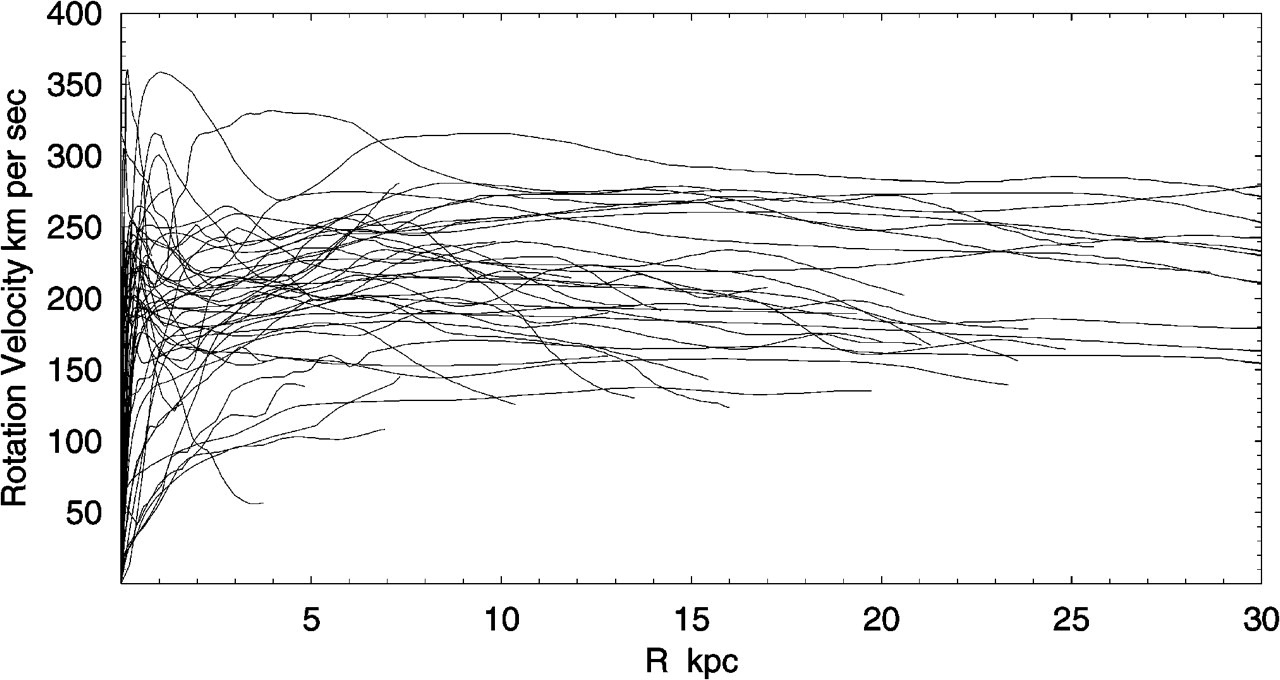
\includegraphics[width=\textwidth]{images/rotation_curves}
\end{sidecaption}
\end{figure}
One of the most tantalizing clues to the nature of dark matter is the so-called 'WIMP miracle' - the remarkable coincidence that the observed dark matter density in the universe can arises naturally from a particle with mass and couplings comparable to the weak scale. This raises the hope that such particles might feasibly be detected at colliders or direct detection experiments.

\section{Dark matter, three ways}\label{dark-matter-three-ways}

\begin{marginfigure}
  \begin{tikzpicture}
    \begin{feynman}
      \vertex (v1) {\(\chi\)};
      \vertex [right=of v1] (v2){\(SM\)};
      \vertex [below=of v1] (v3){\(\chi\)};
      \vertex [right=of v3] (v4){\(SM\)};
      % Placing vertex v between v1 and v4
      \vertex at ($(v1)!0.5!(v4)$) (v);
      \diagram*{
        (v1) -- (v) [blob],
        (v2) -- (v),
        (v3) -- (v),
        (v4) -- (v),
      };
      \draw [->] ($(v1.west) + (-2mm,0)$) -- ($(v3.west) + (-2mm,0)$);
      \draw [->] ($(v1.north) + (0,2mm)$) -- ($(v2.north) + (0,2mm)$);
      \draw [->] ($(v4.south) + (0,-2mm)$) -- ($(v3.south) + (0,-2mm)$);
    \end{feynman}
  \end{tikzpicture}
  \caption{DM detection, three ways}
\end{marginfigure}

There are three main methods of detecting WIMP dark matter. The first, direct detection, involves constructing a well shielded, giant vat of a relatively inert substance, and waiting for dark matter particles to interact with that substance. The second, termed indirect detection, involves searching for signs of dark matter particles annihilating each other in the cosmos. The third method, collider detection, involves producing dark matter through high energy particle collisions and searching for their associated signatures. The first two methods place relatively stringent constraints on the nature of dark matter, but have their own limitations. The smallest interaction cross-section between dark matter and regular matter that direct detection can measure is limited from below by the background of neutrinos from the sun, though there are creative methods that are being developed to deal with this background. Indirect detection suffers from large astrophysical uncertainties. Collider detection, therefore, is competitive with, and can even possibly surpass the other two methods.

\section{Calculation of the thermal relic density}

Assuming that the present-day abundance of WIMP dark matter is explained by a thermal history, the observed density of dark matter, known as the \emph{relic density} sets limits on particle dark matter candidates. We will briefly go over the standard calculation of the thermal relic density.

\newcommand{\fxv}{f(\mathbf{x},\mathbf{v})}

Consider the phase-space density of a single particle dark matter candidate in phase space, given by $\fxv$. That is, the probability of finding the particle with a position of $\mathbf{x}$ and velocity $\mathbf{v}$ is given by $\fxv d^3\mathbf{x}d^3\mathbf{v}$ \footnote{insert references}.
The time evolution of this phase-space density is given by Boltzmann's equation:
\begin{equation}
  \mathbf{L}f = \mathbf{C}f.
\end{equation}
Here, $\mathbf{L}$ is the Liouville operator, which in the non-relativistic limit reduces to 
\begin{equation}
  \mathbf{L}_\text{nr}f = \frac{\partial f}{\partial t} + \mathbf{\dot{x}}\frac{\partial f}{\partial\mathbf{x}} + \mathbf{\dot{v}}\frac{\partial f}{\partial \mathbf{v}} = \frac{d}{dt}
\end{equation}
The general-relativistic version of this operator is obtained by taking the total derivative along a world line parameterized by some affine parameter, say  $\lambda$.
\begin{equation}
  \mathbf{L} = \frac{d}{d\lambda} = \frac{dx^\mu}{d\lambda}\frac{\partial}{\partial x^\mu} + \frac{dp^\mu}{d\lambda}\frac{\partial}{\partial p^\mu}
\end{equation}
We can choose to normalize this parameter as follows:
\begin{equation}
  p^\mu = \frac{dx^\mu}{d\lambda} = m\frac{dx^\mu}{d\tau}
\end{equation}
where $\tau$ is the proper time. With this normalization, the geodesic equation becomes
\begin{equation}
  \frac{dp^\mu}{d\lambda}+\Gamma^{\mu}_{\alpha\beta}p^\alpha p^\beta = 0
\end{equation}
If we assume that there are no external non-gravitational forces, trajectory of the DM particle through phase space will be described by the geodesic. Thus, we can write the general-relativistic Liouville operator as:
\begin{equation}\label{eq:gr_liouville_operator}
  \mathbf{L} = p^\mu\frac{\partial}{\partial x^\mu} - \Gamma^\mu_{\alpha\beta}p^\alpha p^\beta\frac{\partial}{\partial p^\mu}
\end{equation}
The isotropy of the model implies that the phase-space density \emph{f} is devoid of directionality - it will depend only on the energy \emph{E} and time \emph{t}, and can be written as $f(E,t)$. Thus, all the partial derivatives in \eqref{eq:gr_liouville_operator} will vanish except for those corresponding to $\mu = 0$. If the connections $\Gamma^\mu_{\alpha\beta}$ are calculated for the FLRW metric (see \autoref{sec:sm_cosmology}), the Liouville operator simplifies to
\begin{equation}\label{eq:frw_liouville_operator}
  \mathbf{L}f = E\frac{\partial f}{\partial t} + H|\mathbf{p}|^2 \frac{\partial f}{\partial E}
\end{equation}
where $H$ is the Hubble parameter. The number density \emph{n} is given by the integral of $f(E,t)$ over all of phase-space, given by
\begin{align}
  n = 4\pi g\int dp p^2 f(E,t)
\end{align}
where $p = |\mathbf{p}|$, and $g$ is the number of spin degrees of freedom.
Dividing \eqref{eq:frw_liouville_operator} by E and integrating over the momentum coordinates gives us:
\begin{align}
  4\pi g\int dp p^2 \frac{\mathbf{L}f}{E} = 4\pi g\int dp p^2 \left(\frac{\partial f}{\partial t}- H\frac{p^2}{E}\frac{\partial f}{\partial E}\right)
\end{align}
Pulling the partial derivative outside the integral for the first term gives us
\begin{equation}
  \frac{dn}{dt} - 4\pi gH\int dp\frac{p^4}{E}\frac{\partial f}{\partial E}
\end{equation}
We know that $E^2 = p^2 - m^2$, thus $\frac{1}{E}\frac{\partial}{\partial E} = \frac{1}{p}\frac{\partial}{\partial p}$. Substituting this into the previous equation gives us:
\begin{equation}\label{eq:n_dot}
  \dot{n} - 4\pi gH\int dp p^3 \frac{\partial f}{\partial p}
\end{equation}
We can simplify the second term using integration by parts:
\begin{equation}
  \int dp p^3\frac{\partial f}{\partial p} = fp^3|_{0}^\infty - \int dp (3p^2 f)
\end{equation}
The first term on the right hand side of the above equation should evaluate to zero, since the probability of the particle having an infinite momentum must be zero. Substituting this expression into \eqref{eq:n_dot} and simplifying gives us
\begin{equation}\label{eq:simplified_n_density}
  \dot{n}+3Hn = 4\pi g\int \frac{dpp^2}{E}\mathbf{C}f
\end{equation}
The operator \textbf{C} is known as the \emph{collision} operator, and contains the information about how the dark matter particles interact with themselves and other particles. For a process of the form $1+2\rightarrow 3+4$, the collision term (on the right hand side of the above equation) for particle 1 takes the form  
\begin{marginfigure}
  \feynmandiagram[horizontal = chi2 to SM1]{
    {chi1 [particle = \(\chi\)], chi2 [particle = \(\chi\)],
    SM1 [particle = \(SM\)], SM2 [particle = \(SM\)]} -- v [blob],
  };
  \label{fig:dm_annihilation}
  \caption{Dark matter annihilating to SM particles.}
\end{marginfigure}
\begin{equation}\label{eq:collision_term}
  \begin{split}
  &-\sum_\text{spins}\int [f_1 f_2(1\pm f_3)(1\pm f_4)|\mathcal{M}_{12\rightarrow 34}|^2 + f_3 f_4(1\pm f_1)(1\pm f_2)|\mathcal{M}_{34\rightarrow 12}|^2]\\
&\times(2\pi)^4\delta^4(p_1+p_2-p_3-p_4)d\Pi_1 d\Pi_2 d\Pi_3 d\Pi_4
\end{split}
\end{equation}
where
\[d\Pi_i = \frac{d^3 p_i}{(2\pi)^3 2E_i}\]
are phase-space integration factors. This can be simplified considerably by assuming the following:
\begin{itemize}
  \item The early universe is in thermal equilibrium, and thus the phase-space distribution $f$ takes either Fermi-Dirac or Bose-Einstein form.
  \item The temperature of each species, $T_i$ is low enough that the condition $T_i \ll E_i - \mu_i$, where $\mu_i$ is its chemical potential. This means that their phase-space distributions are approximately of the Maxwell-Boltzmann form, and we can neglect the statistical factors: $(1+f)\approx 1$.
\end{itemize}
The amplitude for the forward and backwards processes should be equal:
\[|\mathcal{M}_{12\rightarrow 34}|^2 = |\mathcal{M}_{34\rightarrow 12}|^2 = |\mathcal{M}|^2 \]
Then the expression in \eqref{eq:collision_term} simplifies to
\begin{equation}
-\sum_\text{spins}\int(f_1 f_2 - f_3 f_4)|\mathcal{M}|^2(2\pi)^4\delta(p_1 + p_2 - p_3 - p_4)d\Pi_1 d\Pi_2 d\Pi_3 d\Pi_4
\end{equation}
We can relate the matrix element to the cross section as follows:
\[\sum_\text{spins}|\mathcal{M}_{ij\rightarrow kl}|^2\times(2\pi)^4\delta^4(p_i + p_j - p_k -p_l)d\Pi_jd\Pi_k = 4g_ig_j\sigma_{ij}\sqrt{(p_i\cdot p_j)^2 - (m_im_j)^2}\]
where $\sigma_{ij}$ is the scattering cross section. Let us define the M\o ller velocity,
\[v_\text{M\o l} = \frac{\sqrt{(p_i\cdot p_j)^2 - (m_im_j)^2}}{E_iE_j}\]
Substituting this in the collision term and noting that $f_i(2E_i)d\Pi_i = dn_i$, we get the collision term as
\[g_1\int \mathbf{C}f_1\frac{d^3p_1}{(2\pi)^3} = -\int[(\sigma v_\text{M\o l})_{12}dn_1dn_2 - (\sigma v_\text{M\o l})_{34}dn_3dn_4]\]
The quantity $\sigma v_\text{M\o l}$ is relatively independent of the number densities $n_i$, and thus can be taken outside the integral, to give us
\[\dot{n}_1 + 3Hn_1 = -\langle\sigma v\rangle_{12}n_1n_2 + \langle\sigma v\rangle_{34}n_3n_4.\]
where $v = v_\text{M\o l}$. Let us now apply this result to the specific $2\rightarrow 2$ annihilation case shown in \autoref{fig:dm_annihilation}. The incoming DM particles are identical, with number density \emph{n}. When the DM particles are in equilibrium with the SM particles, a condition known as \emph{detailed balance} holds that relates the number densities and annihilation cross sections for the SM and DM particles:
\[\langle\sigma v\rangle_{12}n^2_\text{eq}=\langle\sigma v\rangle_{34}n_3^\text{eq}n_4^\text{eq}\]
Thus, the Boltzmann equation can be written as
\[\dot{n}+3Hn = \langle\sigma v\rangle (n_\text{eq}^2 - n^2)\]
where $\langle\sigma v\rangle = \langle\sigma v\rangle_{12}$. Intuitively, the number density $n$ will decrease naturally as the universe expands. If we want to focus on the effects of collision, we should define a \emph{comoving number density} $Y = n/s$, where $s$ is the total entropy density of the universe. If the dominant contribution to \emph{s} comes from thermal radiation, then $sa^3$ will be approximately constant. Rewriting the Boltzmann equation in terms of $Y$ gives us
\[\frac{dY}{dt} = \langle\sigma v\rangle s (Y_\text{eq}^2 - Y^2)\]
As the early radiation-dominated universe expanded, it also cooled down. It is expedient to write the above equation in terms of temperature, using the variable $x = m/T$, where \emph{m} is the mass of the DM particle. 
\[\frac{dY}{dx} = -\frac{\langle\sigma v\rangle s}{H(x)x}\]
The thermally averaged cross-section times velocity is given by
\begin{equation}\label{eq:thermal_sigma_v}
  \langle\sigma v\rangle = \frac{\int\sigma vdn_1^\text{eq}dn_2^\text{eq}}{\int dn_1^\text{eq}dn_2^\text{eq}}
  =\frac{\int \sigma v e^{-E_1/T}e^{-E_2/T}d^3p_1d^3p_2}{\int e^{-E_1/T}e^{-E_2/T}d^3p_1d^3p_2}
\end{equation}
The momentum-space volume element in spherical coordinates is
\[d^3p_1d^3p_2 = 4\pi |\mathbf{p}_1|dE_14\pi |\mathbf{p}_2|dE_2\frac{1}{2}d(\cos\theta)\]
where $\theta$ is the angle between the 3-momenta $\mathbf{p}_1$ and $\mathbf{p}_2$. We can then change the integration variables to $E_+, E_-, s$, given by
\begin{align}
  E_+ &= E_1 + E_2\\
  E_- &= E_1 - E_2,\\
  s &= 2m^2 + 2E_1E_2-2\mathbf{p}_1\mathbf{p}_2\cos\theta
\end{align}
Thus the volume element in these variables becomes
\[d^3p_1d^3p_2 = 2\pi^2E_1E_2dE_+dE_-ds\]
And the integration limits become
\begin{align}
  |E_1| &\leq \sqrt{1-\frac{4m^2}{s}}\sqrt{E_+^2 - s}\\
  E_+ &\geq \sqrt{s}\\
  s &\geq 4m^2
\end{align}
With these variables, the numerator in \eqref{eq:thermal_sigma_v} becomes
\begin{align*}
  &2\pi^2\int dE_+\int dE_-\int ds(\sigma v)E_1E_2e^{-E_+/T}\\
  =&4\pi^2\int ds\sigma \frac{1}{2}\sqrt{s(s-4m^2)}\sqrt{1-\frac{4m^2}{s}}\int dE_+e^{-E_+/T}\sqrt{E_+-s}\\
  =&2\pi^2T\int ds\sigma(s-4m^2)\sqrt{s}K_1(\sqrt{s}/T)
\end{align*}
Similarly, the denominator simplifies to $[4\pi m^2TK_2(m/T)]^2$. The functions $K_i$ are modified Bessel functions of order \emph{i}\footnote{The ordinary differential equation
  \begin{equation*}
    x^2\ddot{y} + x\dot{y} - (x^2+n^2)y = 0
  \end{equation*}
  admits solutions of the form $y = c_1 I_n(x) + c_2K_n(x)$. The functions $I_n$ and $K_n$ are known as modified Bessel functions of the first and second kinds, respectively.
}. Thus \eqref{eq:thermal_sigma_v} simplifies to
\[\langle\sigma v\rangle = \frac{1}{8m^4TK_2^2(m/T)}\int_{4m^2}^\infty\sigma(s-4m^2)\sqrt{s}K_1(\sqrt{s}/T)ds\]
In this non-relativistic limit, this simplifies to
\[\langle\sigma v\rangle \approx b_0 + \frac{3}{2}b_1x^{-1} + ...\]
The coefficients $b_0, b_1, ...$ correspond to \emph{s}-wave, \emph{p}-wave annihilation, and so on.

\strictpagecheck
\begin{figure}
  \begin{sidecaption}{Illustration of the freeze-out mechanism}
  % \includegraphics[width=\textwidth]{images/relic_density.pdf}
    %% Creator: Matplotlib, PGF backend
%%
%% To include the figure in your LaTeX document, write
%%   \input{<filename>.pgf}
%%
%% Make sure the required packages are loaded in your preamble
%%   \usepackage{pgf}
%%
%% Figures using additional raster images can only be included by \input if
%% they are in the same directory as the main LaTeX file. For loading figures
%% from other directories you can use the `import` package
%%   \usepackage{import}
%% and then include the figures with
%%   \import{<path to file>}{<filename>.pgf}
%%
%% Matplotlib used the following preamble
%%   \usepackage{fontspec}
%%   \setmonofont{Andale Mono}
%%
\begingroup%
\makeatletter%
\begin{pgfpicture}%
\pgfpathrectangle{\pgfpointorigin}{\pgfqpoint{3.888197in}{2.403038in}}%
\pgfusepath{use as bounding box, clip}%
\begin{pgfscope}%
\pgfsetbuttcap%
\pgfsetmiterjoin%
\definecolor{currentfill}{rgb}{0.941176,0.941176,0.941176}%
\pgfsetfillcolor{currentfill}%
\pgfsetlinewidth{0.000000pt}%
\definecolor{currentstroke}{rgb}{0.941176,0.941176,0.941176}%
\pgfsetstrokecolor{currentstroke}%
\pgfsetdash{}{0pt}%
\pgfpathmoveto{\pgfqpoint{0.000000in}{0.000000in}}%
\pgfpathlineto{\pgfqpoint{3.888197in}{0.000000in}}%
\pgfpathlineto{\pgfqpoint{3.888197in}{2.403038in}}%
\pgfpathlineto{\pgfqpoint{0.000000in}{2.403038in}}%
\pgfpathclose%
\pgfusepath{fill}%
\end{pgfscope}%
\begin{pgfscope}%
\pgfsetbuttcap%
\pgfsetmiterjoin%
\definecolor{currentfill}{rgb}{0.941176,0.941176,0.941176}%
\pgfsetfillcolor{currentfill}%
\pgfsetlinewidth{0.000000pt}%
\definecolor{currentstroke}{rgb}{0.000000,0.000000,0.000000}%
\pgfsetstrokecolor{currentstroke}%
\pgfsetstrokeopacity{0.000000}%
\pgfsetdash{}{0pt}%
\pgfpathmoveto{\pgfqpoint{0.676752in}{0.518611in}}%
\pgfpathlineto{\pgfqpoint{3.738197in}{0.518611in}}%
\pgfpathlineto{\pgfqpoint{3.738197in}{2.253038in}}%
\pgfpathlineto{\pgfqpoint{0.676752in}{2.253038in}}%
\pgfpathclose%
\pgfusepath{fill}%
\end{pgfscope}%
\begin{pgfscope}%
\pgfpathrectangle{\pgfqpoint{0.676752in}{0.518611in}}{\pgfqpoint{3.061445in}{1.734427in}} %
\pgfusepath{clip}%
\pgfsetbuttcap%
\pgfsetroundjoin%
\pgfsetlinewidth{1.003750pt}%
\definecolor{currentstroke}{rgb}{0.796078,0.796078,0.796078}%
\pgfsetstrokecolor{currentstroke}%
\pgfsetdash{}{0pt}%
\pgfpathmoveto{\pgfqpoint{0.815909in}{0.518611in}}%
\pgfpathlineto{\pgfqpoint{0.815909in}{2.253038in}}%
\pgfusepath{stroke}%
\end{pgfscope}%
\begin{pgfscope}%
\pgftext[x=0.815909in,y=0.469999in,,top]{\setmainfont{Minion Pro}\rmfamily\fontsize{10.000000}{12.000000}\selectfont \(\displaystyle {10^{0}}\)}%
\end{pgfscope}%
\begin{pgfscope}%
\pgfpathrectangle{\pgfqpoint{0.676752in}{0.518611in}}{\pgfqpoint{3.061445in}{1.734427in}} %
\pgfusepath{clip}%
\pgfsetbuttcap%
\pgfsetroundjoin%
\pgfsetlinewidth{1.003750pt}%
\definecolor{currentstroke}{rgb}{0.796078,0.796078,0.796078}%
\pgfsetstrokecolor{currentstroke}%
\pgfsetdash{}{0pt}%
\pgfpathmoveto{\pgfqpoint{1.743619in}{0.518611in}}%
\pgfpathlineto{\pgfqpoint{1.743619in}{2.253038in}}%
\pgfusepath{stroke}%
\end{pgfscope}%
\begin{pgfscope}%
\pgftext[x=1.743619in,y=0.469999in,,top]{\setmainfont{Minion Pro}\rmfamily\fontsize{10.000000}{12.000000}\selectfont \(\displaystyle {10^{1}}\)}%
\end{pgfscope}%
\begin{pgfscope}%
\pgfpathrectangle{\pgfqpoint{0.676752in}{0.518611in}}{\pgfqpoint{3.061445in}{1.734427in}} %
\pgfusepath{clip}%
\pgfsetbuttcap%
\pgfsetroundjoin%
\pgfsetlinewidth{1.003750pt}%
\definecolor{currentstroke}{rgb}{0.796078,0.796078,0.796078}%
\pgfsetstrokecolor{currentstroke}%
\pgfsetdash{}{0pt}%
\pgfpathmoveto{\pgfqpoint{2.671330in}{0.518611in}}%
\pgfpathlineto{\pgfqpoint{2.671330in}{2.253038in}}%
\pgfusepath{stroke}%
\end{pgfscope}%
\begin{pgfscope}%
\pgftext[x=2.671330in,y=0.469999in,,top]{\setmainfont{Minion Pro}\rmfamily\fontsize{10.000000}{12.000000}\selectfont \(\displaystyle {10^{2}}\)}%
\end{pgfscope}%
\begin{pgfscope}%
\pgfpathrectangle{\pgfqpoint{0.676752in}{0.518611in}}{\pgfqpoint{3.061445in}{1.734427in}} %
\pgfusepath{clip}%
\pgfsetbuttcap%
\pgfsetroundjoin%
\pgfsetlinewidth{1.003750pt}%
\definecolor{currentstroke}{rgb}{0.796078,0.796078,0.796078}%
\pgfsetstrokecolor{currentstroke}%
\pgfsetdash{}{0pt}%
\pgfpathmoveto{\pgfqpoint{3.599040in}{0.518611in}}%
\pgfpathlineto{\pgfqpoint{3.599040in}{2.253038in}}%
\pgfusepath{stroke}%
\end{pgfscope}%
\begin{pgfscope}%
\pgftext[x=3.599040in,y=0.469999in,,top]{\setmainfont{Minion Pro}\rmfamily\fontsize{10.000000}{12.000000}\selectfont \(\displaystyle {10^{3}}\)}%
\end{pgfscope}%
\begin{pgfscope}%
\pgftext[x=2.207475in,y=0.282222in,,top]{\setmainfont{Minion Pro}\rmfamily\fontsize{10.000000}{12.000000}\selectfont x}%
\end{pgfscope}%
\begin{pgfscope}%
\pgfpathrectangle{\pgfqpoint{0.676752in}{0.518611in}}{\pgfqpoint{3.061445in}{1.734427in}} %
\pgfusepath{clip}%
\pgfsetbuttcap%
\pgfsetroundjoin%
\pgfsetlinewidth{1.003750pt}%
\definecolor{currentstroke}{rgb}{0.796078,0.796078,0.796078}%
\pgfsetstrokecolor{currentstroke}%
\pgfsetdash{}{0pt}%
\pgfpathmoveto{\pgfqpoint{0.676752in}{0.518611in}}%
\pgfpathlineto{\pgfqpoint{3.738197in}{0.518611in}}%
\pgfusepath{stroke}%
\end{pgfscope}%
\begin{pgfscope}%
\pgftext[x=0.340139in,y=0.469166in,left,base]{\setmainfont{Minion Pro}\rmfamily\fontsize{10.000000}{12.000000}\selectfont \(\displaystyle {10^{-5}}\)}%
\end{pgfscope}%
\begin{pgfscope}%
\pgfpathrectangle{\pgfqpoint{0.676752in}{0.518611in}}{\pgfqpoint{3.061445in}{1.734427in}} %
\pgfusepath{clip}%
\pgfsetbuttcap%
\pgfsetroundjoin%
\pgfsetlinewidth{1.003750pt}%
\definecolor{currentstroke}{rgb}{0.796078,0.796078,0.796078}%
\pgfsetstrokecolor{currentstroke}%
\pgfsetdash{}{0pt}%
\pgfpathmoveto{\pgfqpoint{0.676752in}{0.843816in}}%
\pgfpathlineto{\pgfqpoint{3.738197in}{0.843816in}}%
\pgfusepath{stroke}%
\end{pgfscope}%
\begin{pgfscope}%
\pgftext[x=0.340139in,y=0.794371in,left,base]{\setmainfont{Minion Pro}\rmfamily\fontsize{10.000000}{12.000000}\selectfont \(\displaystyle {10^{-2}}\)}%
\end{pgfscope}%
\begin{pgfscope}%
\pgfpathrectangle{\pgfqpoint{0.676752in}{0.518611in}}{\pgfqpoint{3.061445in}{1.734427in}} %
\pgfusepath{clip}%
\pgfsetbuttcap%
\pgfsetroundjoin%
\pgfsetlinewidth{1.003750pt}%
\definecolor{currentstroke}{rgb}{0.796078,0.796078,0.796078}%
\pgfsetstrokecolor{currentstroke}%
\pgfsetdash{}{0pt}%
\pgfpathmoveto{\pgfqpoint{0.676752in}{1.169021in}}%
\pgfpathlineto{\pgfqpoint{3.738197in}{1.169021in}}%
\pgfusepath{stroke}%
\end{pgfscope}%
\begin{pgfscope}%
\pgftext[x=0.426945in,y=1.119576in,left,base]{\setmainfont{Minion Pro}\rmfamily\fontsize{10.000000}{12.000000}\selectfont \(\displaystyle {10^{1}}\)}%
\end{pgfscope}%
\begin{pgfscope}%
\pgfpathrectangle{\pgfqpoint{0.676752in}{0.518611in}}{\pgfqpoint{3.061445in}{1.734427in}} %
\pgfusepath{clip}%
\pgfsetbuttcap%
\pgfsetroundjoin%
\pgfsetlinewidth{1.003750pt}%
\definecolor{currentstroke}{rgb}{0.796078,0.796078,0.796078}%
\pgfsetstrokecolor{currentstroke}%
\pgfsetdash{}{0pt}%
\pgfpathmoveto{\pgfqpoint{0.676752in}{1.494226in}}%
\pgfpathlineto{\pgfqpoint{3.738197in}{1.494226in}}%
\pgfusepath{stroke}%
\end{pgfscope}%
\begin{pgfscope}%
\pgftext[x=0.426945in,y=1.444782in,left,base]{\setmainfont{Minion Pro}\rmfamily\fontsize{10.000000}{12.000000}\selectfont \(\displaystyle {10^{4}}\)}%
\end{pgfscope}%
\begin{pgfscope}%
\pgfpathrectangle{\pgfqpoint{0.676752in}{0.518611in}}{\pgfqpoint{3.061445in}{1.734427in}} %
\pgfusepath{clip}%
\pgfsetbuttcap%
\pgfsetroundjoin%
\pgfsetlinewidth{1.003750pt}%
\definecolor{currentstroke}{rgb}{0.796078,0.796078,0.796078}%
\pgfsetstrokecolor{currentstroke}%
\pgfsetdash{}{0pt}%
\pgfpathmoveto{\pgfqpoint{0.676752in}{1.819431in}}%
\pgfpathlineto{\pgfqpoint{3.738197in}{1.819431in}}%
\pgfusepath{stroke}%
\end{pgfscope}%
\begin{pgfscope}%
\pgftext[x=0.426945in,y=1.769987in,left,base]{\setmainfont{Minion Pro}\rmfamily\fontsize{10.000000}{12.000000}\selectfont \(\displaystyle {10^{7}}\)}%
\end{pgfscope}%
\begin{pgfscope}%
\pgfpathrectangle{\pgfqpoint{0.676752in}{0.518611in}}{\pgfqpoint{3.061445in}{1.734427in}} %
\pgfusepath{clip}%
\pgfsetbuttcap%
\pgfsetroundjoin%
\pgfsetlinewidth{1.003750pt}%
\definecolor{currentstroke}{rgb}{0.796078,0.796078,0.796078}%
\pgfsetstrokecolor{currentstroke}%
\pgfsetdash{}{0pt}%
\pgfpathmoveto{\pgfqpoint{0.676752in}{2.144636in}}%
\pgfpathlineto{\pgfqpoint{3.738197in}{2.144636in}}%
\pgfusepath{stroke}%
\end{pgfscope}%
\begin{pgfscope}%
\pgftext[x=0.371582in,y=2.095192in,left,base]{\setmainfont{Minion Pro}\rmfamily\fontsize{10.000000}{12.000000}\selectfont \(\displaystyle {10^{10}}\)}%
\end{pgfscope}%
\begin{pgfscope}%
\pgftext[x=0.284583in,y=1.385824in,,bottom,rotate=90.000000]{\setmainfont{Minion Pro}\rmfamily\fontsize{10.000000}{12.000000}\selectfont Number density}%
\end{pgfscope}%
\begin{pgfscope}%
\pgfpathrectangle{\pgfqpoint{0.676752in}{0.518611in}}{\pgfqpoint{3.061445in}{1.734427in}} %
\pgfusepath{clip}%
\pgfsetbuttcap%
\pgfsetroundjoin%
\pgfsetlinewidth{0.501875pt}%
\definecolor{currentstroke}{rgb}{0.000000,0.560784,0.835294}%
\pgfsetstrokecolor{currentstroke}%
\pgfsetdash{}{0pt}%
\pgfpathmoveto{\pgfqpoint{0.815909in}{2.169617in}}%
\pgfpathlineto{\pgfqpoint{0.854276in}{2.172283in}}%
\pgfpathlineto{\pgfqpoint{0.889306in}{2.173719in}}%
\pgfpathlineto{\pgfqpoint{0.979150in}{2.175356in}}%
\pgfpathlineto{\pgfqpoint{1.052567in}{2.174113in}}%
\pgfpathlineto{\pgfqpoint{1.114645in}{2.170883in}}%
\pgfpathlineto{\pgfqpoint{1.168423in}{2.166198in}}%
\pgfpathlineto{\pgfqpoint{1.230509in}{2.158266in}}%
\pgfpathlineto{\pgfqpoint{1.284292in}{2.148878in}}%
\pgfpathlineto{\pgfqpoint{1.331735in}{2.138379in}}%
\pgfpathlineto{\pgfqpoint{1.374174in}{2.127003in}}%
\pgfpathlineto{\pgfqpoint{1.421619in}{2.111801in}}%
\pgfpathlineto{\pgfqpoint{1.464061in}{2.095722in}}%
\pgfpathlineto{\pgfqpoint{1.502454in}{2.078933in}}%
\pgfpathlineto{\pgfqpoint{1.544164in}{2.058022in}}%
\pgfpathlineto{\pgfqpoint{1.581959in}{2.036425in}}%
\pgfpathlineto{\pgfqpoint{1.616510in}{2.014260in}}%
\pgfpathlineto{\pgfqpoint{1.653398in}{1.987800in}}%
\pgfpathlineto{\pgfqpoint{1.687190in}{1.960798in}}%
\pgfpathlineto{\pgfqpoint{1.722629in}{1.929380in}}%
\pgfpathlineto{\pgfqpoint{1.755201in}{1.897461in}}%
\pgfpathlineto{\pgfqpoint{1.788949in}{1.861044in}}%
\pgfpathlineto{\pgfqpoint{1.820087in}{1.824169in}}%
\pgfpathlineto{\pgfqpoint{1.852078in}{1.782741in}}%
\pgfpathlineto{\pgfqpoint{1.884562in}{1.736697in}}%
\pgfpathlineto{\pgfqpoint{1.914621in}{1.690231in}}%
\pgfpathlineto{\pgfqpoint{1.945041in}{1.639139in}}%
\pgfpathlineto{\pgfqpoint{1.975594in}{1.583423in}}%
\pgfpathlineto{\pgfqpoint{2.006097in}{1.523247in}}%
\pgfpathlineto{\pgfqpoint{2.046019in}{1.438903in}}%
\pgfpathlineto{\pgfqpoint{2.075332in}{1.378767in}}%
\pgfpathlineto{\pgfqpoint{2.090930in}{1.351591in}}%
\pgfpathlineto{\pgfqpoint{2.104305in}{1.332491in}}%
\pgfpathlineto{\pgfqpoint{2.117250in}{1.317734in}}%
\pgfpathlineto{\pgfqpoint{2.131333in}{1.305156in}}%
\pgfpathlineto{\pgfqpoint{2.146424in}{1.294647in}}%
\pgfpathlineto{\pgfqpoint{2.165234in}{1.284466in}}%
\pgfpathlineto{\pgfqpoint{2.187240in}{1.275231in}}%
\pgfpathlineto{\pgfqpoint{2.214411in}{1.266374in}}%
\pgfpathlineto{\pgfqpoint{2.248005in}{1.257923in}}%
\pgfpathlineto{\pgfqpoint{2.288492in}{1.250103in}}%
\pgfpathlineto{\pgfqpoint{2.339286in}{1.242653in}}%
\pgfpathlineto{\pgfqpoint{2.402047in}{1.235782in}}%
\pgfpathlineto{\pgfqpoint{2.480964in}{1.229477in}}%
\pgfpathlineto{\pgfqpoint{2.580563in}{1.223853in}}%
\pgfpathlineto{\pgfqpoint{2.707903in}{1.218991in}}%
\pgfpathlineto{\pgfqpoint{2.874923in}{1.214952in}}%
\pgfpathlineto{\pgfqpoint{3.102571in}{1.211807in}}%
\pgfpathlineto{\pgfqpoint{3.435820in}{1.209606in}}%
\pgfpathlineto{\pgfqpoint{3.599040in}{1.209052in}}%
\pgfpathlineto{\pgfqpoint{3.599040in}{1.209052in}}%
\pgfusepath{stroke}%
\end{pgfscope}%
\begin{pgfscope}%
\pgfpathrectangle{\pgfqpoint{0.676752in}{0.518611in}}{\pgfqpoint{3.061445in}{1.734427in}} %
\pgfusepath{clip}%
\pgfsetbuttcap%
\pgfsetroundjoin%
\pgfsetlinewidth{0.501875pt}%
\definecolor{currentstroke}{rgb}{0.988235,0.309804,0.188235}%
\pgfsetstrokecolor{currentstroke}%
\pgfsetdash{{5.600000pt}{2.400000pt}}{0.000000pt}%
\pgfpathmoveto{\pgfqpoint{0.815909in}{2.170262in}}%
\pgfpathlineto{\pgfqpoint{0.854276in}{2.172283in}}%
\pgfpathlineto{\pgfqpoint{0.889306in}{2.173719in}}%
\pgfpathlineto{\pgfqpoint{0.979150in}{2.175356in}}%
\pgfpathlineto{\pgfqpoint{1.052567in}{2.174113in}}%
\pgfpathlineto{\pgfqpoint{1.114645in}{2.170883in}}%
\pgfpathlineto{\pgfqpoint{1.168423in}{2.166198in}}%
\pgfpathlineto{\pgfqpoint{1.230509in}{2.158266in}}%
\pgfpathlineto{\pgfqpoint{1.284292in}{2.148878in}}%
\pgfpathlineto{\pgfqpoint{1.331735in}{2.138379in}}%
\pgfpathlineto{\pgfqpoint{1.374174in}{2.127003in}}%
\pgfpathlineto{\pgfqpoint{1.421619in}{2.111801in}}%
\pgfpathlineto{\pgfqpoint{1.464061in}{2.095722in}}%
\pgfpathlineto{\pgfqpoint{1.502454in}{2.078933in}}%
\pgfpathlineto{\pgfqpoint{1.544164in}{2.058022in}}%
\pgfpathlineto{\pgfqpoint{1.581959in}{2.036425in}}%
\pgfpathlineto{\pgfqpoint{1.616510in}{2.014260in}}%
\pgfpathlineto{\pgfqpoint{1.653398in}{1.987800in}}%
\pgfpathlineto{\pgfqpoint{1.687190in}{1.960798in}}%
\pgfpathlineto{\pgfqpoint{1.722629in}{1.929380in}}%
\pgfpathlineto{\pgfqpoint{1.755201in}{1.897461in}}%
\pgfpathlineto{\pgfqpoint{1.788949in}{1.861044in}}%
\pgfpathlineto{\pgfqpoint{1.820087in}{1.824169in}}%
\pgfpathlineto{\pgfqpoint{1.852078in}{1.782740in}}%
\pgfpathlineto{\pgfqpoint{1.884562in}{1.736694in}}%
\pgfpathlineto{\pgfqpoint{1.914621in}{1.690223in}}%
\pgfpathlineto{\pgfqpoint{1.945041in}{1.639112in}}%
\pgfpathlineto{\pgfqpoint{1.975594in}{1.583321in}}%
\pgfpathlineto{\pgfqpoint{2.006097in}{1.522817in}}%
\pgfpathlineto{\pgfqpoint{2.036403in}{1.457575in}}%
\pgfpathlineto{\pgfqpoint{2.066399in}{1.387575in}}%
\pgfpathlineto{\pgfqpoint{2.095998in}{1.312801in}}%
\pgfpathlineto{\pgfqpoint{2.125135in}{1.233244in}}%
\pgfpathlineto{\pgfqpoint{2.155215in}{1.144444in}}%
\pgfpathlineto{\pgfqpoint{2.184554in}{1.050811in}}%
\pgfpathlineto{\pgfqpoint{2.214411in}{0.947862in}}%
\pgfpathlineto{\pgfqpoint{2.243374in}{0.840052in}}%
\pgfpathlineto{\pgfqpoint{2.272565in}{0.722875in}}%
\pgfpathlineto{\pgfqpoint{2.301803in}{0.596299in}}%
\pgfpathlineto{\pgfqpoint{2.320838in}{0.508611in}}%
\pgfpathlineto{\pgfqpoint{2.320838in}{0.508611in}}%
\pgfusepath{stroke}%
\end{pgfscope}%
\begin{pgfscope}%
\pgfsetrectcap%
\pgfsetmiterjoin%
\pgfsetlinewidth{3.011250pt}%
\definecolor{currentstroke}{rgb}{0.941176,0.941176,0.941176}%
\pgfsetstrokecolor{currentstroke}%
\pgfsetdash{}{0pt}%
\pgfpathmoveto{\pgfqpoint{0.676752in}{0.518611in}}%
\pgfpathlineto{\pgfqpoint{0.676752in}{2.253038in}}%
\pgfusepath{stroke}%
\end{pgfscope}%
\begin{pgfscope}%
\pgfsetrectcap%
\pgfsetmiterjoin%
\pgfsetlinewidth{3.011250pt}%
\definecolor{currentstroke}{rgb}{0.941176,0.941176,0.941176}%
\pgfsetstrokecolor{currentstroke}%
\pgfsetdash{}{0pt}%
\pgfpathmoveto{\pgfqpoint{3.738197in}{0.518611in}}%
\pgfpathlineto{\pgfqpoint{3.738197in}{2.253038in}}%
\pgfusepath{stroke}%
\end{pgfscope}%
\begin{pgfscope}%
\pgfsetrectcap%
\pgfsetmiterjoin%
\pgfsetlinewidth{3.011250pt}%
\definecolor{currentstroke}{rgb}{0.941176,0.941176,0.941176}%
\pgfsetstrokecolor{currentstroke}%
\pgfsetdash{}{0pt}%
\pgfpathmoveto{\pgfqpoint{0.676752in}{0.518611in}}%
\pgfpathlineto{\pgfqpoint{3.738197in}{0.518611in}}%
\pgfusepath{stroke}%
\end{pgfscope}%
\begin{pgfscope}%
\pgfsetrectcap%
\pgfsetmiterjoin%
\pgfsetlinewidth{3.011250pt}%
\definecolor{currentstroke}{rgb}{0.941176,0.941176,0.941176}%
\pgfsetstrokecolor{currentstroke}%
\pgfsetdash{}{0pt}%
\pgfpathmoveto{\pgfqpoint{0.676752in}{2.253038in}}%
\pgfpathlineto{\pgfqpoint{3.738197in}{2.253038in}}%
\pgfusepath{stroke}%
\end{pgfscope}%
\end{pgfpicture}%
\makeatother%
\endgroup%

  \end{sidecaption}
\end{figure}
